% Introduce detector, location, basic info (e.g., chamber count)
% What is the technology
% Anatomy of a chamber
% How are they arranged in the barrel/endcap
% What do they measure
% Coverage
% Performance

Complementing the DT chambers and CSCs are the Resistive Plate Chambers (RPCs) located in both the MB and ME (shown in Fig.~\ref{fig:RPC}). RPCs have two naming conventions, depending on the region of the detector they occupy: in the barrel, ``RBn$\pm$w,'' and in the endcaps, ``RE$\pm$n/m,'' where ($\pm$)n denotes the MB or ME$\pm$ station (1-4), $\pm$w the MB wheel (1-5), and m the ME ring (1, 2, or 3 in RB$\pm$1; 1or 2 in all other stations). Pseudorapidity coverage by the RPCs overlaps with the other muon subsytems at $0.0 < |\eta| < 1.9$. In stations RB1 and RB2, two RPCs sandwich each DT chamber, while in RB3 and RB4, anywhere from one to four RPCs (depending on the station and sector) are layered on the inside of a single DT chamber. This leads to 480 total RPCs in the barrel. In the endcaps, RPCs are mounted to the opposite side of a yoke disk as the CSCs, forming alternating layers of CSCs and RPCs, and totalling 576 RPCs in the endcaps. Each RPC is a \SI{2}{mm} double-gap chamber, using Bakalite (a high pressure laminate) electrodes, operated in avalanche mode (see the diagram in Fig.~\ref{fig:RPCDiagram}). Electrode strips are longitudinally-running and segemnted into two or three parts, depending on the station/sector. A RPC detector is optimized to record accurate timing and fast triggering, as well as identification the associated bunch crossing for a given muon track. Compared to the DTs and CSCs, RPCs have a coarse-grain spatial resolution of only \SIrange{0.8}{1.3}{cm}, but provide excellent timing resolution at \SI{1.5}{ns}.

\begin{figure}[H]
    \centering
    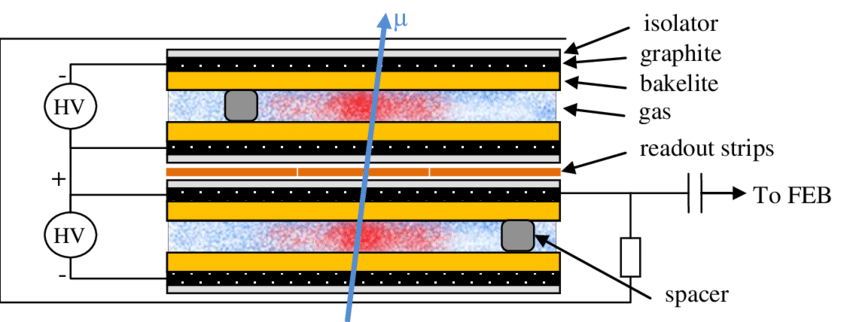
\includegraphics[width=\textwidth]{Images/CMS/RPCDiagram.png}
    \caption{A diagram of an RPC.}
    \label{fig:RPCDiagram}
\end{figure}


\begin{figure}[H]
    \centering
    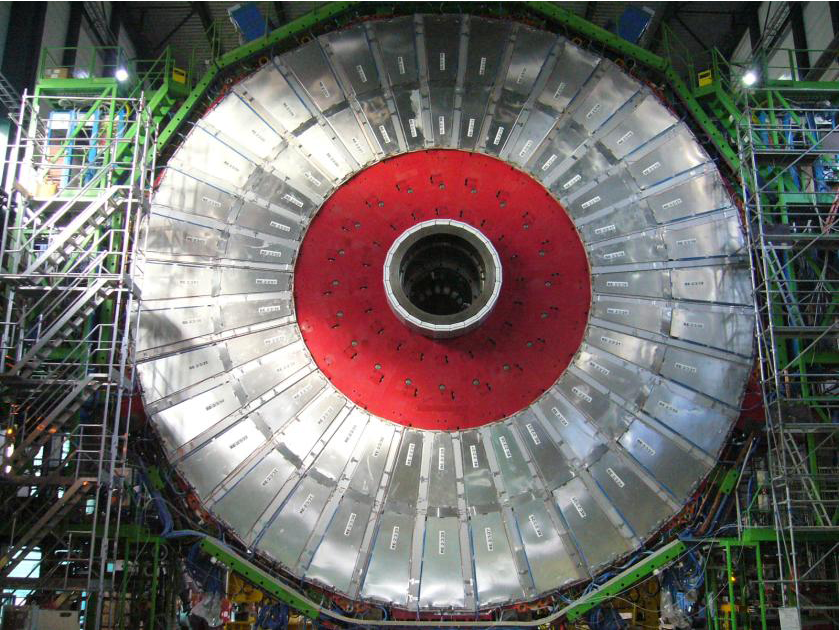
\includegraphics[width=1\textwidth]{Images/CMS/RE.png}
    \caption{A photograph of RPCs mounted to the second endcap station.}
    \label{fig:RPC}
\end{figure}